\subsubsection{Data prefetching}
The data prefetching on \textit{EmporioLambda} makes use of Next.js\textsubscript{G} pre-rendering.\\
More precisely, Next.js\textsubscript{G} allows the use of 2 types of pre-rendering:
\begin{itemize}
\item \textbf{static generation\textsubscript{G}:} the system generates the HTML\textsubscript{G} at build time. The pre-rendered HTML\textsubscript{G} is then reused on each request;
\begin{figure}[H]
\centering
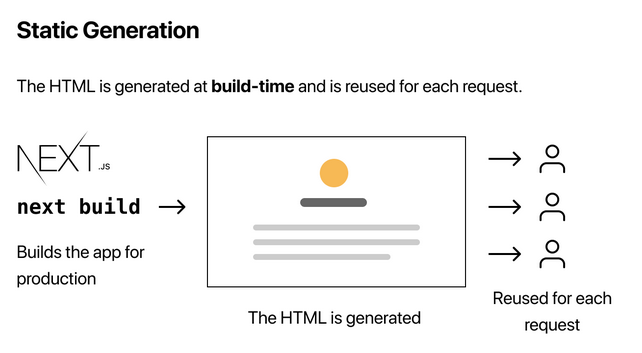
\includegraphics[scale=0.70]{res/Architettura/Frontend/img/staticGeneration}\\
\caption{Static generation\textsubscript{G} scheme}
\end{figure}
\vspace{0.7cm}
\item \textbf{server-side rendering\textsubscript{G}:} the system generates the HTML\textsubscript{G} on each request.
\begin{figure}[H]
\centering
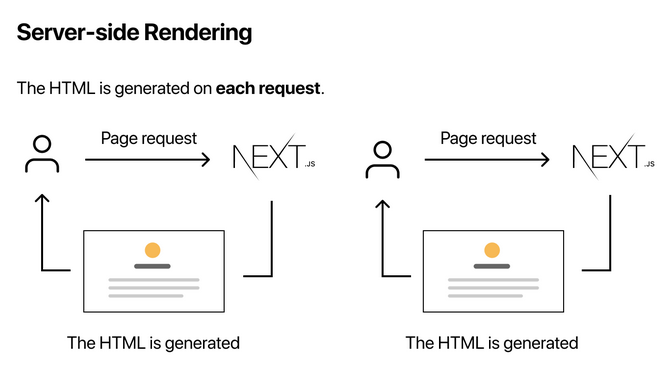
\includegraphics[scale=0.70]{res/Architettura/Frontend/img/serverSideRendering}\\
\caption{Server-side rendering\textsubscript{G} scheme}
\end{figure}
\vspace{0.7cm}
\end{itemize}
One difference between these 2 pre-rendering methods is the response time of the website.
Static generation\textsubscript{G} is faster than server-side rendering so the second one should only be used when necessary. Each page can use a different type of prefetch.\\
In \textit{EmporioLambda} each page prefetches data using these 2 methods:
\begin{itemize}
\item \textbf{getStaticProps:} a function that returns a GetStaticProps object, which indicates that the page will use static generation\textsubscript{G};
\item \textbf{getServerSideProps:} a function that return a GetServerSideProps object, which indicates that the page will use server-side rendering\textsubscript{G}. It will thus render again after receiving new data.
\end{itemize}
Both functions return a Typescript\textsubscript{G} object called props which contains the needed data. This object will be passed to the component part of the Front-end\textsubscript{G} module.\\
More information about Next.js\textsubscript{G} pre-rendering can be found on this page:\\
\url{https://nextjs.org/learn/basics/data-fetching/two-forms}.\\
All of the pages in \textit{EmporioLambda} use server-side rendering\textsubscript{G}.